\section{What the quaternionic lift adds}

The \(3\)-D helicoid--catenoid picture already carries the incompleteness
slogan (Figure~\ref{fig:formal}).
The Hopf version is worth writing only if the fiber is used.

\paragraph{Diagram, not extra symbols.}
Base \(S^{2}\) is catalog-visible.
Fiber \(S^{1}\) is the remainder.
The map \(h\) is the catalog projection.

\begin{center}
\begin{tikzpicture}[
  font=\small,
  every node/.style={align=center},
  arr/.style={-{Stealth[length=2mm]}, thick}
]
  \node[draw, circle, minimum size=1.55cm] (s1) {\(S^{1}\)\\[-1pt]\scriptsize fiber};
  \node[draw, circle, minimum size=1.7cm, below=0.85cm of s1] (s3) {\(S^{3}\)};
  \node[draw, circle, minimum size=1.55cm, right=2.6cm of s3] (s2) {\(S^{2}\)\\[-1pt]\scriptsize base};
  \draw[arr] (s1) -- node[left, font=\scriptsize] {life} (s3);
  \draw[arr] (s3) -- node[above] {\(h\)} (s2);
  \node[font=\scriptsize, below=0.28cm of s2] {catalog-visible};
  \node[font=\scriptsize, right=0.15cm of s1, xshift=0.2cm] {remainder:\\[-1pt]the base cannot invert};
\end{tikzpicture}
\end{center}

\begin{model}[Hopf lift of the helicoid--catenoid generator]
Same split, different stage.
Dynamics on \(S^{3}\) and on the gauged Hopf lattice.
Spine input only:
\(S^{3}\subset\mathbb{H}\),
\(h:S^{3}\to S^{2}\),
\(N(q)=q\bar q\).
See \url{https://github.com/kinaar8340/qga}.
\end{model}

\paragraph{Definitions.}
\begin{align}
\XO(q)
&= iq,
\label{eq:qga-XO}\\
\QO\,p
&:= -\operatorname{div}_{S^{3}}(\XO\,p),
\label{eq:qga-QO}\\
\QC\,p
&:= \sum_{q'\sim q}
      \bigl[w(q\mid q')p(q')-w(q'\mid q)p(q)\bigr],
\label{eq:qga-QC}\\
\frac{\partial p(q,t)}{\partial t}
&= Qp
= \QO\,p + \sigma(Z)\,\QC\,p.
\label{eq:qga-master}
\end{align}
Here \(q'\sim q\) means neighbors in the gauged Hopf lattice
(or topograph edges).
That \(\sim\)\, is QGA Open Problem~1:
the kernel \(w\) is exogenous.
It is not claimed to be Hatcher's Farey lift.

Life on this stage is transport along the structure-group fiber of
QGA's \(h\): left common-phase \(q\mapsto e^{i\theta}q\), generated by
the right-invariant field~\eqref{eq:qga-XO}.
The left-invariant field \(q\mapsto qi\) generates the fiber of the other
Hopf map \(q\mapsto qi\bar q\) and is not used.
No extra invariance claim is a term in \(Q\).

Mass conservation is Lemma~\ref{lem:mass} with \(d\Psi\) replaced by
the Riemannian measure \(d\mu\) on \(S^{3}\).
Markov is Lemma~\ref{lem:markov}: \(Q^{\ast}1=0\), and the jump piece
is Kolmogorov forward.
The remainder is the Spine fact (Hopf remainder).
\(N(q)=1\) is the standing constraint on this stage.
Linking of fibers is a property of \(h\), not something the ODE proves.

\paragraph{Symbols.}
\begin{itemize}[leftmargin=1.4em,itemsep=2pt,topsep=4pt,parsep=0pt]
  \item \(q\in S^{3}\subset\mathbb{H}\),
        \(h:S^{3}\to S^{2}\),
        \(N(q)=q\bar q=1\).
  \item \(\XO(q)=iq\): right-invariant fiber field of \(h\) (life).
  \item \(w(q\mid q')\ge 0\): gauge / adjacency kernel on \(\Lambda\).
  \item \(\sigma(Z)\ge 0\): catalog gate (\(\sigma=0\): pure fiber life).
\end{itemize}

\begin{center}
\textit{The catalog needs the life; the life is not the catalog.}
\end{center}

\begin{figure}[H]
  \centering
  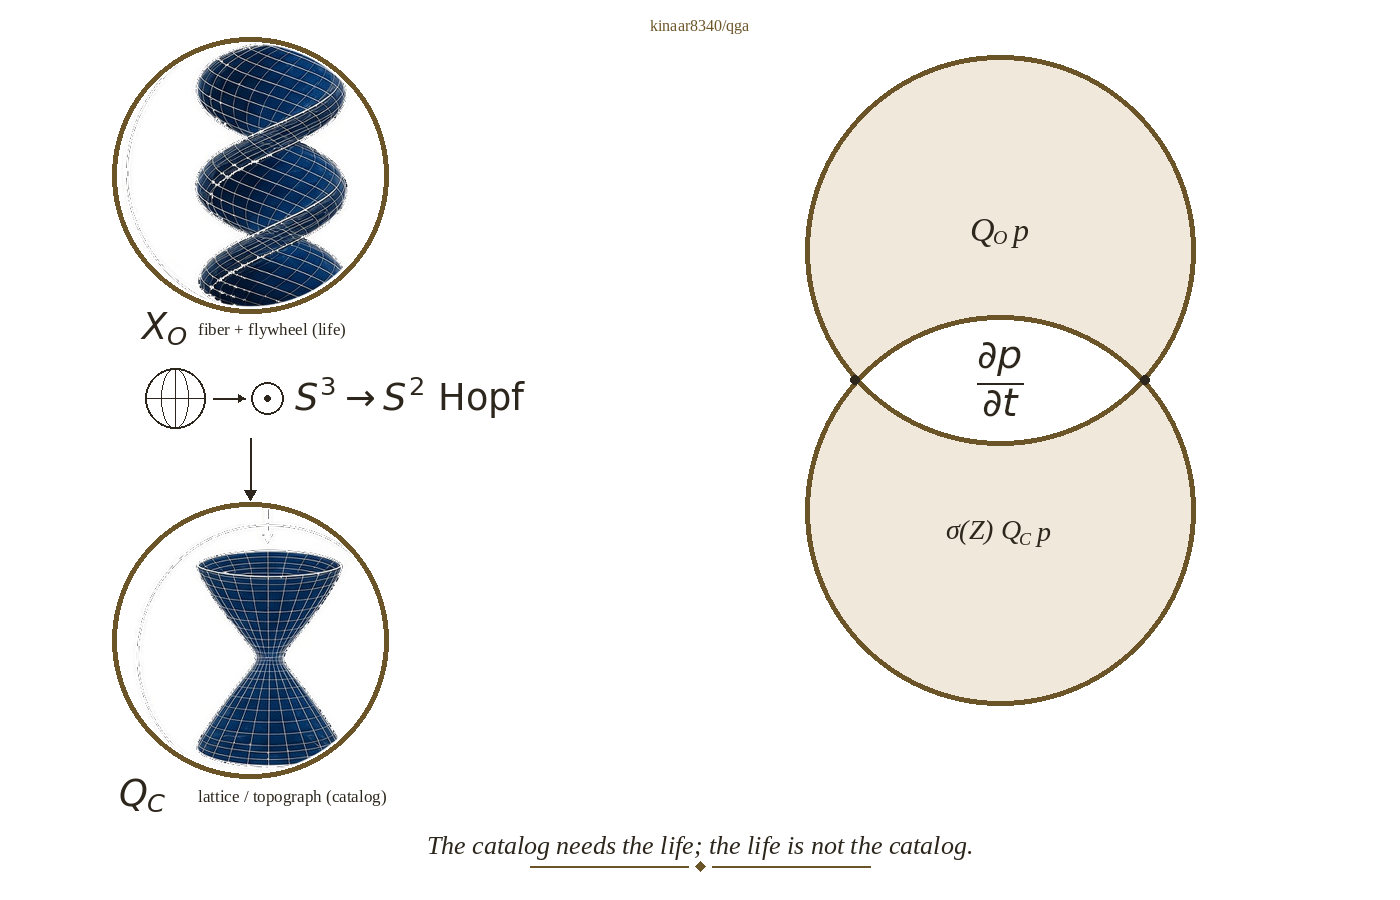
\includegraphics[width=0.88\linewidth]{../fig/qga-full-object.png}
  \caption{QGA full object, still a Model.
  \(\XO\) runs on the fiber;
  \(\QC\) runs on lattice / topograph edges;
  \(h:S^{3}\to S^{2}\) is the catalog projection that cannot invert the fiber.}
  \label{fig:qga}
\end{figure}

\paragraph{Comparison.}
\(\QO\) is advection in both objects (vector field on \(\Psi\),
fiber field on \(S^{3}\)).
\(\QC\) is the jump catalog in both (integral kernel, then lattice sum).
The lift changes the \emph{stage}
(\(S^{3}\), Hopf fiber, Hopf linking as a property of \(h\)),
not the \emph{split}.
